\documentclass[tikz,border=10pt]{standalone}
\usepackage[utf8]{inputenc}
\usepackage[T1]{fontenc}
\usepackage[english]{babel}
\usepackage{graphicx}
\usepackage{amsmath,amssymb}
\usepackage{tikz}
\usepackage{hyperref}
\usepackage{geometry}
\usepackage{fancyhdr}
\usepackage{listings}
\usepackage{color}
\usepackage{caption}
\usepackage{booktabs}
\usepackage{longtable}
\usepackage{float}
\usepackage{array}
\usepackage{subfigure}
\usepackage{multirow}
\usepackage{multicol}
\usepackage[acronym]{glossaries}
\usepackage{xcolor}
\usetikzlibrary{shapes.geometric,arrows,positioning,calc,fit}

\begin{document}
\pagecolor{white}
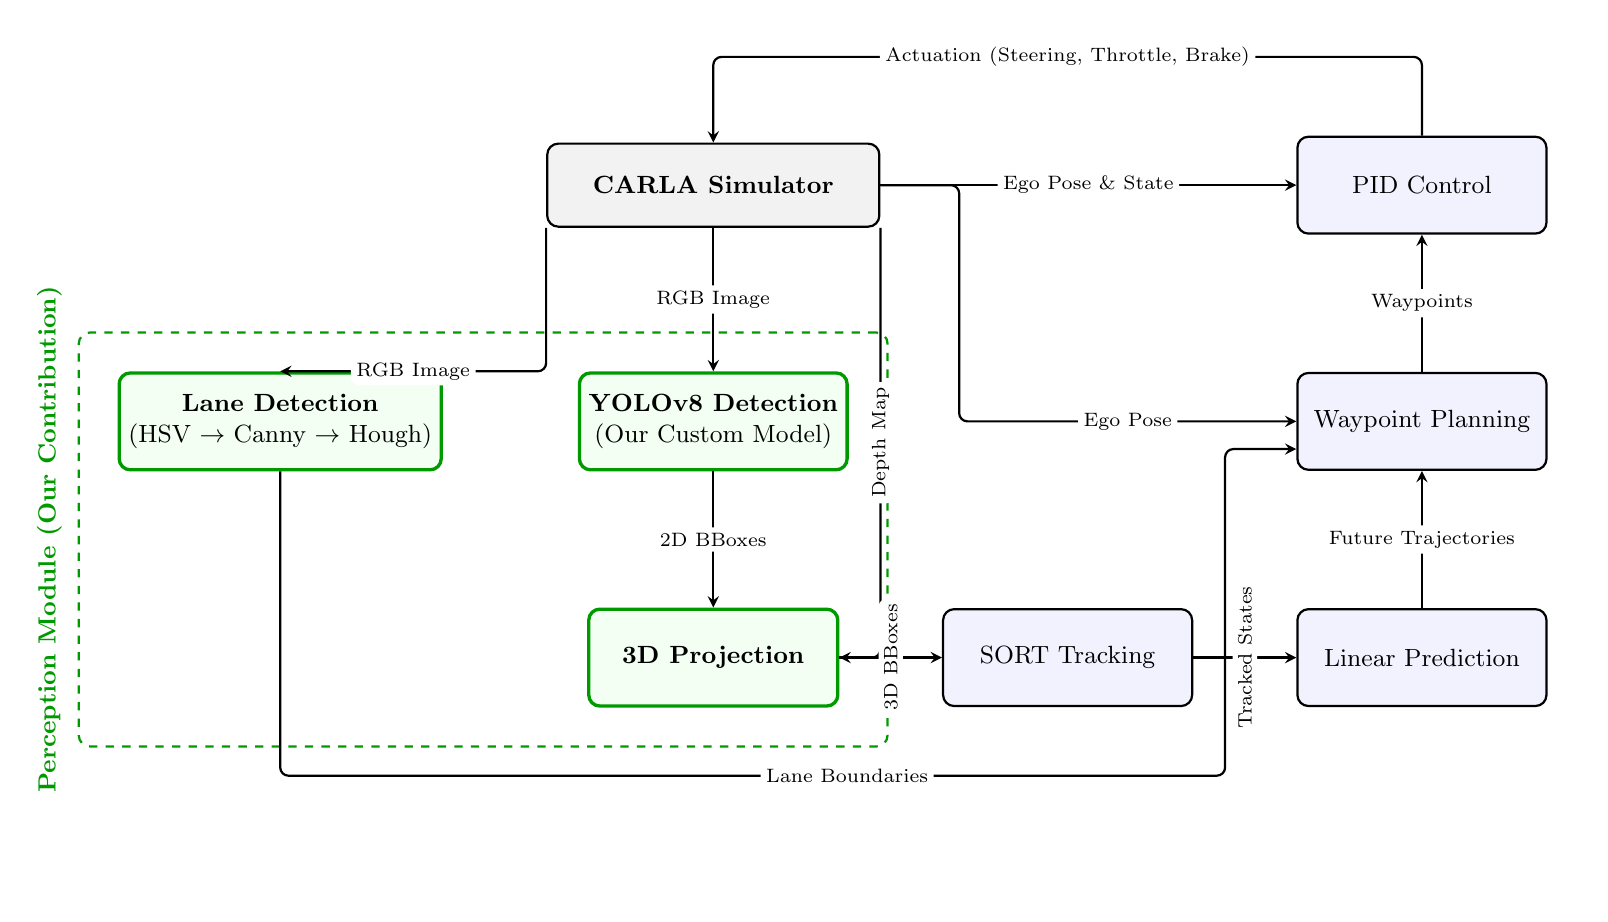
\begin{tikzpicture}[>=stealth, thick]
        \tikzset{
            sensor/.style={draw, fill=gray!10, rectangle, minimum height=3em, minimum width=12em, rounded corners, align=center, font=\small\bfseries},
            module/.style={draw, fill=blue!5, rectangle, minimum height=3.5em, minimum width=9em, rounded corners, align=center, font=\small},
            highlight/.style={draw=green!60!black, fill=green!5, rectangle, minimum height=3.5em, minimum width=9em, rounded corners, align=center, font=\small, line width=1.2pt},
            io/.style={font=\scriptsize, align=center, fill=white, inner sep=2pt},
            line/.style={draw, ->, >=stealth, thick, rounded corners=3pt}
        }
        
        % Simulator
        \node [sensor] (carla) at (2, 0) {CARLA Simulator};
        
        % Perception Module
        \node [highlight] (lane) at (-3.5, -3) {\textbf{Lane Detection}\\(HSV $\rightarrow$ Canny $\rightarrow$ Hough)};
        \node [highlight] (yolo) at (2, -3) {\textbf{YOLOv8 Detection}\\(Our Custom Model)};
        \node [highlight] (proj) at (2, -6) {\textbf{3D Projection}};
        
        % Grouping Perception
        \node[draw=green!60!black, dashed, rounded corners, fit=(lane) (yolo) (proj), inner sep=14pt] (perception_box) {};
        \node[green!60!black, font=\small\bfseries, rotate=90, anchor=south, yshift=2pt] at (perception_box.west) {Perception Module (Our Contribution)};
        
        % Downstream Modules
        \node [module] (sort) at (6.5, -6) {SORT Tracking};
        \node [module] (pred) at (11, -6) {Linear Prediction};
        \node [module] (plan) at (11, -3) {Waypoint Planning};
        \node [module] (control) at (11, 0) {PID Control};
        
        % Connections from CARLA
        \draw [line] (carla.south) -- node[io] {RGB Image} (yolo.north);
        \draw [line] (carla.south west) |- node[io, near end] {RGB Image} (lane.north);
        \draw [line] (carla.south east) |- node[io, near start, rotate=90] {Depth Map} (proj.east);
        \draw [line] (carla.east) -- node[io] {Ego Pose \& State} (control.west);
        \draw [line] (carla.east) -- +(1,0) |- node[io, near end] {Ego Pose} (plan.west);
        
        % Internal Perception Connections
        \draw [line] (yolo.south) -- node[io] {2D BBoxes} (proj.north);
        
        % Perception to Downstream
        \draw [line] (proj.east) -- node[io, rotate=90] {3D BBoxes} (sort.west);
        \draw [line] (lane.south) |- node[io, pos=0.8] {Lane Boundaries} (8.5, -7.5) |- ($(plan.west) + (0,-10pt)$);
        
        % Downstream connections
        \draw [line] (sort.east) -- node[io, rotate=90] {Tracked States} (pred.west);
        \draw [line] (pred.north) -- node[io] {Future Trajectories} (plan.south);
        \draw [line] (plan.north) -- node[io] {Waypoints} (control.south);
        
        % Feedback to CARLA
        \draw [line] (control.north) -- +(0,1) -| node[io, near start] {Actuation (Steering, Throttle, Brake)} (carla.north);
        
        \useasboundingbox (-5, -9) rectangle (13, 2);
\end{tikzpicture}
\end{document}